\chapter{RESULTADOS E DISCUSSÕES}\label{chap:resultados}

A escala de cada diagrama de fase das misturas binárias são distintas, pelo fato de que cada ácido graxo ou álcool possui ponto de fusão distintos como podemos verificar nas seções \ref{sec:1} até \ref{sec:4}.

\section{Estudos de casos.}

\subsection{Sistema 1: Ácido Mirístico e Ácido Esteárico}\label{sistema1}

Na Figura \ref{fig:11} o diagrama de fase foi determinado pelos modelos termodinâmicos \textit{MA}, \textit{MS} e \textit{Wilson} implementado no \textit{GAMS} e o gráfico gerado pelo \textit{PyCharm} com biblioteca do \textit{R}. Os dados experimentais comparativos foram obtidos por COSTA 2009 por experimentos com o método de DSC.
\begin{figure}[H]
	\centering
	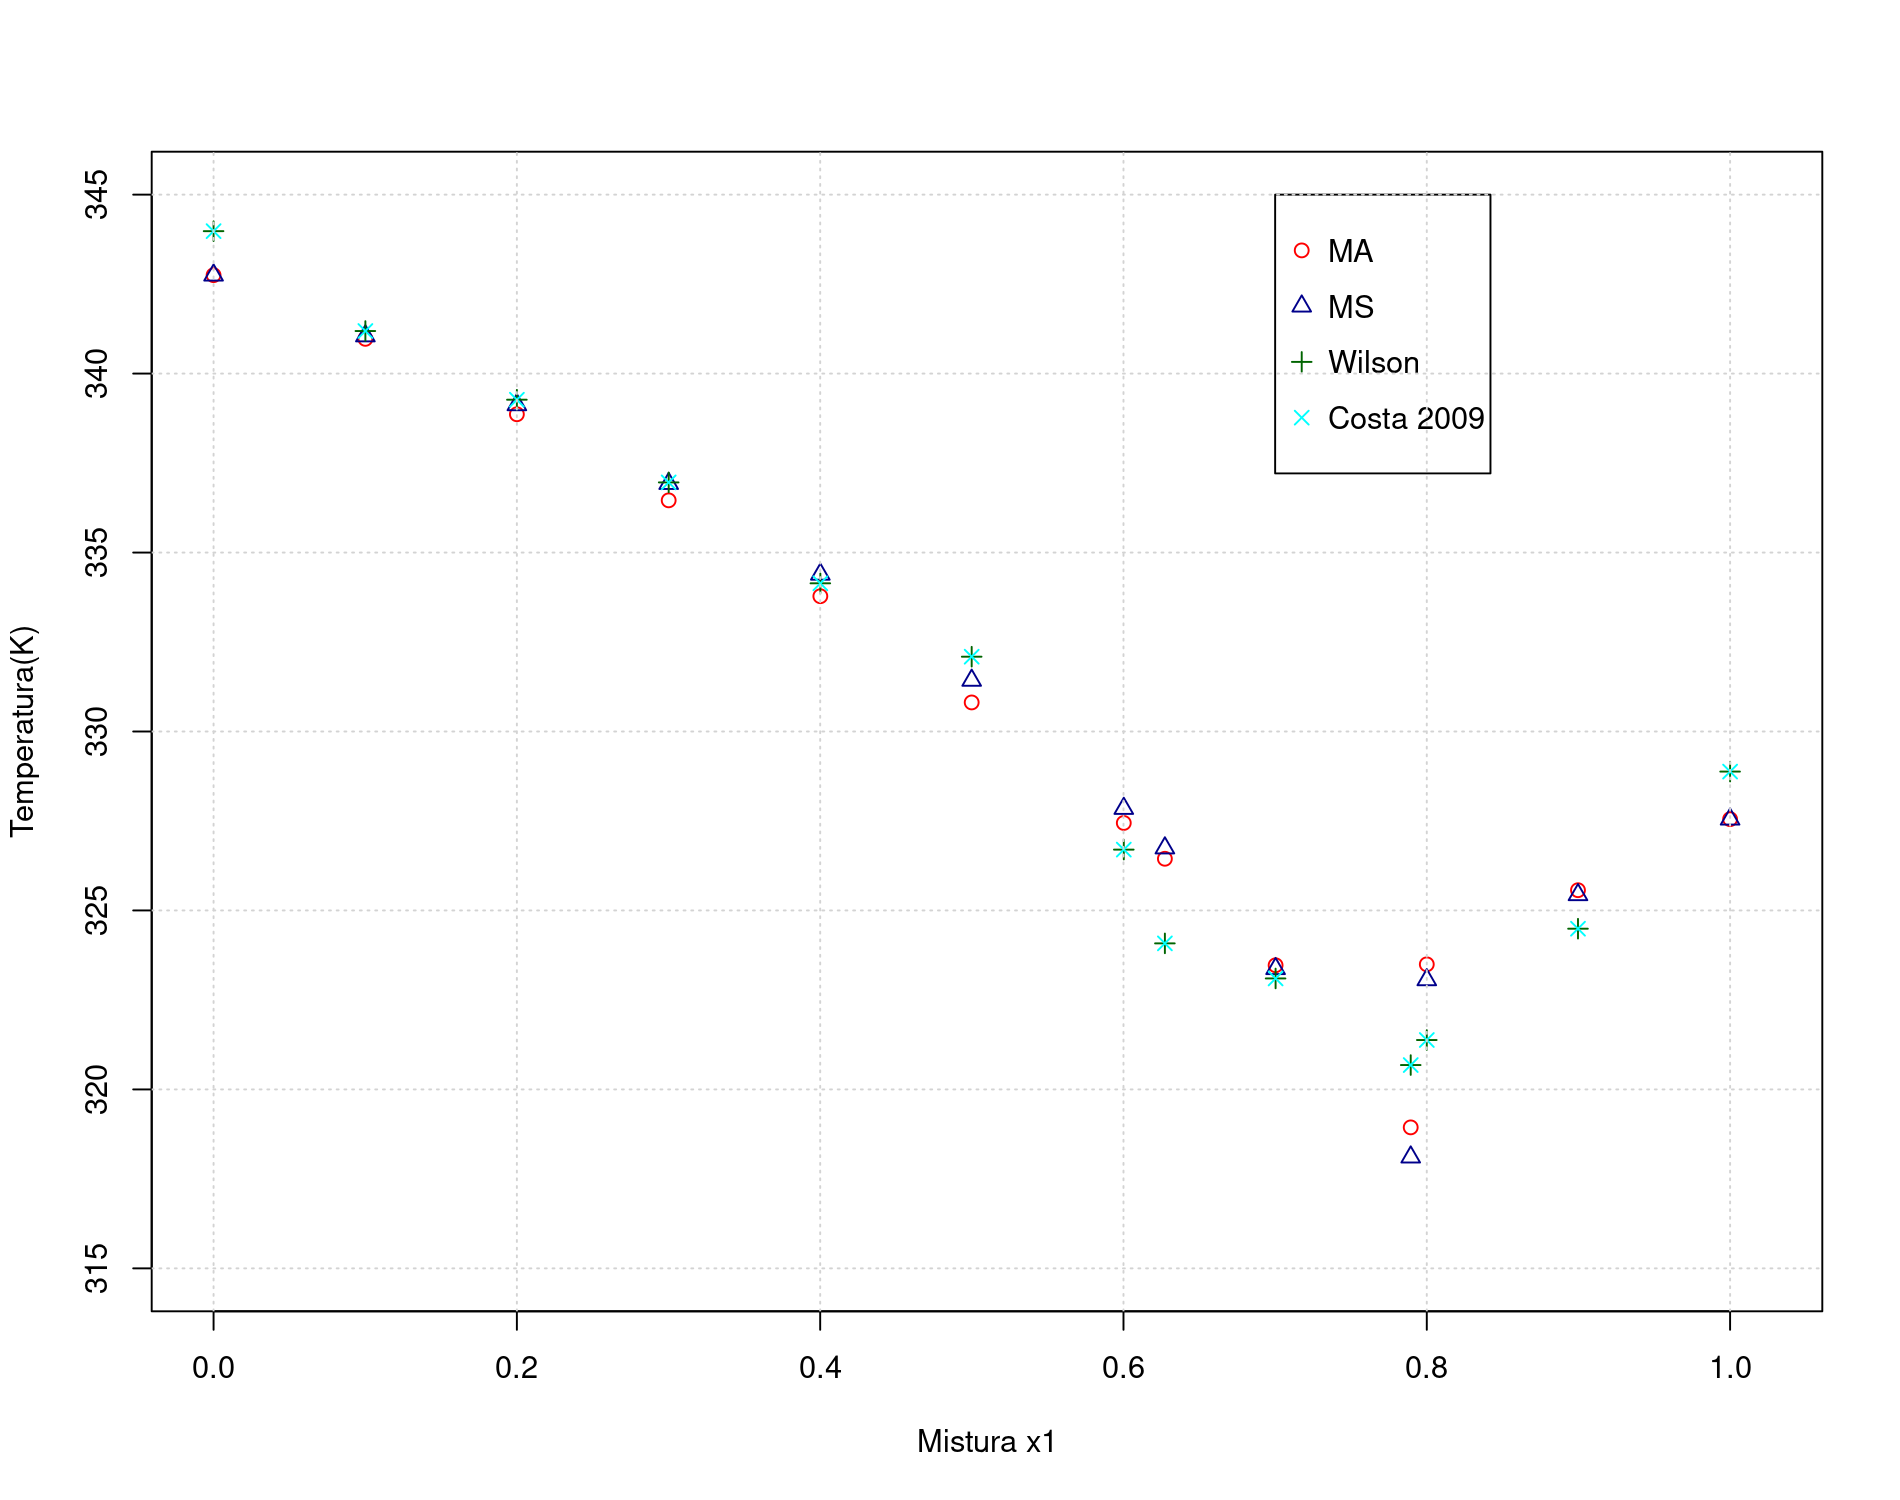
\includegraphics[width=1.06\linewidth 
	%,height=0.4\textheight
	]{dados/figuras/Miristico_estearico.png}
	\caption[Diagrama do equilíbrio sólido-líquido para mistura Ácido Mirístico e Ácido Esteárico]{Diagrama do equilíbrio sólido-líquido para mistura Ácido Mirístico(1) e Ácido Esteárico(2) (\textit{PyCharm}/$R$)}
	\label{fig:3}
\end{figure}

\section{Coeficiente de Determinação}

A propriedade do coeficiente de determinação é que:
\begin{itemize}
    \item $R^2\in [0;1]$
    \item $R^2=1$, $VD$ é explicada pela variação de $VI$ em 100\%
    \item $R^2=0$, $VI$ não tem influencia sobre $VD$.
\end{itemize}

O valor do $R^2$ é calculado pela fórmula
\begin{equation}
    R^2=\frac{\left(\displaystyle\sum_{i=1}^{n}x_i\cdot y_i-n\cdot\overline{x}\cdot\overline{y}\right)^2}{\left(\displaystyle\sum_{i=1}^{n}x_i^2-n\cdot\overline{x}^2\right)\times\left(\displaystyle\sum_{i=1}^{n}y_i^2-n\cdot\overline{y}^2\right)}
\end{equation}
em que $n$ quantidade de elementos da variável $VD$ ou $VI$, $x_i\in VI$ e $y_i\in VD$.
\begin{equation}
    \overline{x}=\frac{\displaystyle\sum_{i=1}^{n}x_i}{n}
\end{equation}
e
\begin{equation}
    \overline{y}=\frac{\displaystyle\sum_{i=1}^{n}y_i}{n}
\end{equation}

%\begin{center}
    %Coeficiente de determinação da variável dependente  técnicas de %DSC e variáveis independentes MA, MS ou Wilson
%\end{center}
\begin{table}[H]
    \caption{Coeficiente de Determinação}
    \centering
    \begin{tabular}{l|p{3cm}p{3cm}p{3cm}}
    %\multicolumn{4}{c}{\textbf{Coeficiente de determinação da variável dependente  técnicas de DSC e variáveis}}  \\ 
    %\multicolumn{4}{c}{\textbf{independentes MA, MS ou Wilson}} \\ 
    \hline
         & $R^2$ MA & $R^2$ MS & $R^2$ Wilson \\
    \hline
    Ac. Mirístico e Ac. Esteárico  & 0.9756  & 0.9706 & 0.9708 \\
    Ac. Palmítico e Ac. Esteárico  & 0.9699  & 0.8005 & 0.7040 \\
    %Ac. Palmítico e Ac. Esteárico  & 0.4955  & 0.5355 & 0.5057 \\
    Hexadecanol e Ac. Mirístico  & 0.2427  & 0.2328 & 0.2133 \\
    Hexadecanol e Tetradecanol  & 0.9804  & 0.9310 & 0.9887 \\
    Ac. Esteárico e Ac. Linoleico  & 0.1483  & 0.5592 & 0.8745 \\
    Ac. Palmítico e Ac. Linoleico  & 0.7490  & 0.5602 & 0.0000 \\
    \end{tabular}
    \label{tab:1}
\end{table}

